\section{Versuchsaufbau}
\label{sec:Versuchsaufbau}

Der Versuchsaufbau besteht im wesentlichen aus einer Kupfer-Rötgenröhre,
einem LiF-Kistall und einem Geiger-Müller-Zählrohr.\\
Alle Bauteile sind im Rötgengerät aus \autoref{Abb:Rötgengerät} verbaut.
Die Maschine wird per Computer bedient.

\begin{figure}
    \centering
    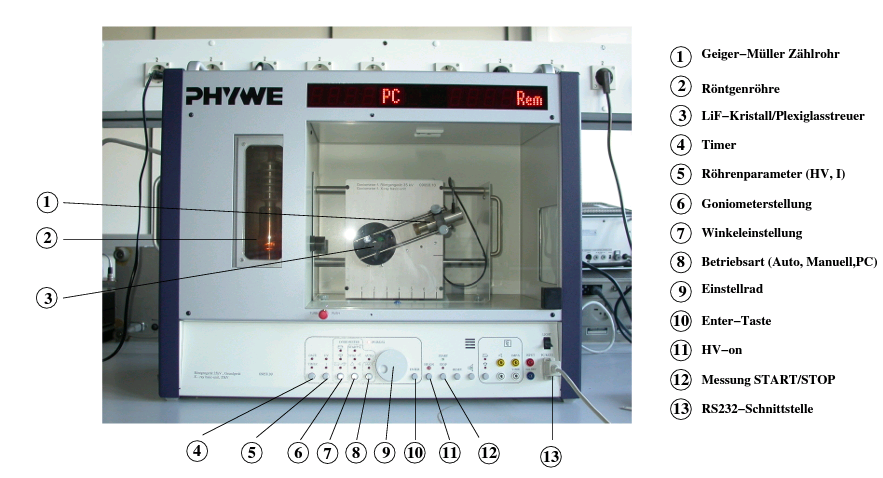
\includegraphics[width=0.7\textwidth]{Bilder/Röntgengerät.png}
    \caption{Aufgenommenes Photo des Röntgengeräts mit Beschriftung der einzelnen Bestandteile \cite{sample}.}
    \label{Abb:Rötgengerät}
\end{figure}

Auf dem Rechner kann das Röntgengerät ausgewählt werden, und eine Messart,
Kristallwinkel, Integrationszeit, Beschleunigungsspannung und Emissionsstrom 
gewählt werden.\\
In alles folgenden Versuchreihen wird eine Beschleunigungsspannung von 
$U_{\mathrm{B}} = 35 \si{\kilo\volt}$ und ein Emissionsstrom von $I = 1 \si{\milli\ampere}$
verwendet.\\

\section{Durchführung}
\label{sec:Durchführung}

\subsection{Überprüfung der Bragg Bedingung}

Bei diesem Versuchsteil wird ein fester Kristallwinkel
von $\theta = 14 ^\circ$, ein Winkelbereich des Zählrohrs
von $\alpha_{\mathrm{GM}} = 26 ^\circ$ bis $\alpha_{\mathrm{GM}} = 30 ^\circ$
mit einem WInkelzuwachs von $\Delta \alpha = 0.1 ^\circ$ und eine 
Integrationszeit von $\Delta t = 5 \si{\second}$ eingestellt.\\

\subsection{Das Emissionsspektrum einer Cu-Röntgenröhre}

Hier wird nun der 2:1 Koppelmodus verwendet und in einem Winkelbereich
von $ 4 ^\circ \leq \theta \leq 26 ^\circ$ in $0.2 ^\circ$
-Schritten gemessen. Die Integrationszeit bleibt gleich.\\
Danach wird noch einmal ein Detailspektrum der $K_{\alpha}$- und $K_{\beta}$-Linien
in einem geeigneten Winkelbereich aufgenommen. Der WInkelzuwachs soll $\Delta \theta = 0.1 ^\circ$
betragen und die Integrationszeit gleich bleiben bei 5 Sekunden.\\

\subsection{Absorptionsspektrum}

Bei diesem Versuchsaufbau werden Zink und vier weitere Absorber
mit einer Ordnungszahl zwischen 30 und 50 verwendet und auf das Geiger-
Müller-Zählrohr gespannt.\\
Es wird eine Integrationszeit von 20 Sekunden eingestellt und einem WInkelzuwachs
von $0.1 ^\circ$-Schritten.
